\chapter{Amortised structures: stacks, deques, sparse tables}\label{ch:amort}
\index{amortised analysis}\index{monotonic stack}\index{monotonic deque}
\index{sparse table}\index{square-root decomposition}

Chapter~5's prefix tables answer questions about an array that never
changes. This chapter is about structures whose cost is invisible
per-operation but bounded per-\emph{element}: a monotonic stack that
finds every position's nearest smaller neighbour in one pass, a deque
that answers sliding-window minima in $O(n)$, a sparse table that
answers static range minimums in $O(1)$ after an $O(n \log n)$ build,
and a square-root split that trades theory for simplicity. The shared
idea is amortisation --- charge each index once for all the work it
will ever cause, and the total is linear no matter how expensive a
single step looks. After this chapter you will recognise the
pop-everything-until pattern, argue its bound by counting pushes, and
pick the right static-range structure for the operation's algebra.

% from-zero:begin
\begin{rulebox}[Before you start]
Chapters~1, 3 and~5. \emph{Recap:} \texttt{stack} means ``last in, first out''; \texttt{deque} means ``add or remove at either end.'' Think of a stack of plates (you only touch the top one) and a queue at a shop where you may also join or leave from the front. Both are one line of C++ (\texttt{stack<int>}, \texttt{deque<int>}).
\end{rulebox}
\begin{wins}[After this chapter you can]
\begin{itemize}
\item argue that a loop with a nested loop is still $O(n)$ because each element is pushed and popped once;
\item find the nearest smaller (or larger) element to the left of every position in one pass;
\item compute every sliding-window minimum in $O(n)$ with a deque;
\item build a sparse table and answer range-minimum queries in $O(1)$.
\end{itemize}
\end{wins}
\begin{principle}[How to think about this]
Some loops look slow because one loop sits inside another, but when you count the \emph{total} work across the whole run, each element is touched a fixed number of times. That is amortised thinking: judge the cost of the whole process, not of one step. The structures here all keep a tidy ``waiting list'' of candidates, and throw away anything that can never be the answer again.
\end{principle}
% from-zero:end

\section{Amortised analysis: each element pays once}\label{sec:amort}
\index{amortised analysis!accounting}

A worst-case bound per operation can be badly pessimistic for a whole
sequence: if each array index is pushed onto a stack at most once and
popped at most once, then $n$ operations cost at most $2n$ stack
touches --- a single push can trigger many pops, but those pops were
\emph{pre-paid} by earlier pushes. This accounting view (charge the
element, not the call) is the licence for every structure in this
chapter: where a per-call bound would say $O(n^2)$, the per-element
bound says $O(n)$.

\section{The monotonic stack: nearest smaller everywhere}\label{sec:monostack}
\index{monotonic stack!nearest smaller}

Keep a stack of indices whose values are strictly increasing. When
position $i$ arrives, pop every index whose value is $\ge a_i$ ---
they can never again be the \emph{nearest} smaller answer, because
$a_i$ is both smaller and closer. The surviving top is $i$'s answer;
push $i$. Every index enters once and leaves once, so the whole pass
is $O(n)$ amortised (Figure~\ref{fig:stackpop}).

\begin{lstlisting}[language=C++,caption={\texttt{monostack.h}: nearest
smaller to the left, and mirrored right.},label={lst:monostack}]
\end{lstlisting}
\lstinputlisting{code/monostack.h}

\begin{example}[CSES \emph{Nearest Smaller Values}]\label{ex:nsv}
For each position, the nearest earlier position with a smaller value
--- $n \le 2\cdot10^5$.
\par\smallskip
\textbf{Strategy.} Per-position search is $O(n^2)$. The amortised
insight: once $a_i$ undercuts an earlier entry, that entry is dead for
every later query --- delete it on sight. What remains is exactly the
monotone stack.
\par\smallskip
\begin{solution}
\lstinputlisting{code/nsv.cpp}
Real output (CSES sample $\{2,5,1,4,8,3,2,5\}$):
\begin{lstlisting}[numbers=none]
0 1 0 3 4 3 3 7
\end{lstlisting}
\end{solution}
\end{example}

\begin{figure}[ht]\centering
\begin{tikzpicture}[font=\footnotesize]
% F6.1 NSV pop trace on {2,5,1,4}: 3 frames.
% frame1: after 2,5 pushed; frame2: 1 pops both; frame3: 4 pushes on 1.
\begin{scope}
  \node[draw=slate,minimum width=0.6cm,font=\tiny] at (0,0) {2};
  \node[draw=slate,minimum width=0.6cm,font=\tiny] at (0,0.5) {5};
  \node[font=\tiny,right] at (0.5,0.25) {stack: 2,5};
  \node[font=\tiny] at (0.3,-0.5) {seen 2,5};
\end{scope}
\begin{scope}[xshift=3.2cm]
  \node[draw=slate,draw=gray,minimum width=0.6cm,font=\tiny] (p1) at (0,0) {2};
  \node[draw=slate,draw=gray,minimum width=0.6cm,font=\tiny] (p2) at (0,0.5) {5};
  \draw[red,thick] (p1.south west)--(p1.north east) (p1.north west)--(p1.south east)
    (p2.south west)--(p2.north east) (p2.north west)--(p2.south east);
  \node[font=\tiny,right] at (0.5,0.25) {1 pops both};
  \node[font=\tiny] at (0.3,-0.5) {next: 1};
\end{scope}
\begin{scope}[xshift=6.4cm]
  \node[draw=slate,fill=accentsoft,minimum width=0.6cm,font=\tiny] at (0,0) {1};
  \node[draw=slate,minimum width=0.6cm,font=\tiny] at (0,0.5) {4};
  \node[font=\tiny,right] at (0.5,0.25) {4's answer = 1's idx};
  \node[font=\tiny] at (0.3,-0.5) {stack: 1,4};
\end{scope}
\node[align=left,text width=3.6cm,font=\tiny] at (10.6,0)
  {each index enters once,\\ leaves once: the pops\\ are pre-paid};
\end{tikzpicture}

\caption{The stack pop trace on $\{2,5,1,4\}$. Notice the popped
entries are \emph{gone}, not skipped: $1$ is closer and smaller than
either, so both can never answer again.}
\label{fig:stackpop}
\end{figure}

\begin{example}[Largest rectangle in a histogram]\label{ex:histogram}
\index{histogram!largest rectangle}
Heights $h_0,\dots,h_{n-1}$; find the largest rectangle that fits
under the skyline.
\par\smallskip
\textbf{Strategy.} Every candidate rectangle has a \emph{limiting
bar} --- its shortest bar --- so try each bar as the limiter: how far
can bar $i$ extend? Exactly until the first smaller bar on each side.
Nearest-smaller to left and right is two monotonic-stack passes.
\par\smallskip
\begin{solution}
\lstinputlisting{code/histogram.cpp}
Real output (heights $\{2,1,5,6,2,3\}$ --- bar~2's rays reach the
first smaller bars, Figure~\ref{fig:histogram}):
\begin{lstlisting}[numbers=none]
best area 10 from bar 2 (height 5, spans [2,3])
\end{lstlisting}
\end{solution}
\end{example}

\begin{figure}[ht]\centering
\begin{tikzpicture}[font=\footnotesize,x=0.5cm,y=0.22cm]
% F6.2 histogram {2,1,5,6,2,3}: bar2's rays to first-smaller bounds.
\foreach \i/\h in {0/2,1/1,2/5,3/6,4/2,5/3}
  \draw[fill=graybg,draw=slate] (\i,0) rectangle (\i+0.9,\h);
\draw[fill=accentsoft,draw=slate] (2,0) rectangle (3.8,5);
\draw[-{stealth},amber,thick] (2.45,5.4) -- (1.4,5.4);
\draw[-{stealth},amber,thick] (2.45,5.4) -- (4.0,5.4);
\node[font=\tiny] at (1.0,6.1) {first smaller left};
\node[font=\tiny] at (4.6,6.1) {first smaller right};
\node[font=\tiny] at (3,-1.6) {bar 2 (height 5): spans $[2,3]$, area $5\cdot2=10$};
\end{tikzpicture}

\caption{Bar 2's horizontal reach ends at the first smaller bar on
each side. Notice the optimal rectangle is pinned by \emph{one}
limiting bar --- which is why trying every bar suffices.}
\label{fig:histogram}
\end{figure}

\begin{exercise}[easy]\label{exr:amort}
The pop loop inside the push is not $O(1)$ --- one push may pop $k$
entries. Argue in one sentence why the total over $n$ pushes is still
$O(n)$.
\end{exercise}

\section{The monotonic deque: sliding-window minimum}\label{sec:monodeque}
\index{monotonic deque!sliding window}

The same pop-until pattern slides a window: the deque keeps candidate
indices in increasing value order, front = current minimum. New index
$i$ pops every back entry with $a_{\text{back}} \ge a_i$ (same
dead-on-arrival argument), then the front drops when it leaves the
window. Each index enters and exits once: $O(n)$ for all windows.

\begin{lstlisting}[language=C++,caption={\texttt{monodeque.h}: window
minimums in $O(n)$.},label={lst:monodeque}]
\end{lstlisting}
\lstinputlisting{code/monodeque.h}

\begin{example}[CSES \emph{Sliding Window Minimum}]\label{ex:slide}
Window size $k$ over a generated array up to $n=10^7$; report the xor
of all window minimums.
\par\smallskip
\textbf{Strategy.} $O(nk)$ is impossible at $10^7$. The deque is the
only structure that retires entries \emph{both} by value (a newer,
smaller element wins) and by age (the window forgets) --- and it is
linear.
\par\smallskip
\begin{solution}
\lstinputlisting{code/sliding_min.cpp}
Real output (CSES sample, generator $x{=}3,a{=}7,b{=}1,c{=}11$,
array $\{3,0,1,8,2,4,7,6\}$, $k{=}5$, minimums $0,0,1,2$):
\begin{lstlisting}[numbers=none]
3
\end{lstlisting}
\end{solution}
\end{example}

\begin{figure}[ht]\centering
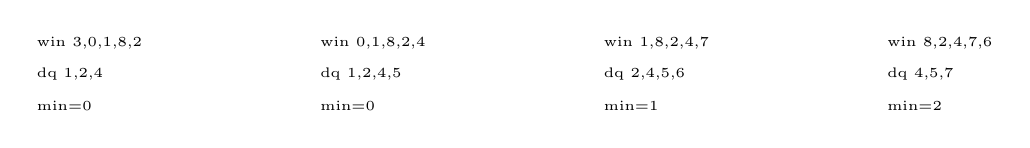
\begin{tikzpicture}[font=\footnotesize]
% F6.3 deque slide on {3,0,1,8,2,4,7,6}, k=5: real index traces.
% dq lists the index stack after each window closes.
\foreach \f/\w/\dq/\mn in {0/{3,0,1,8,2}/{1,2,4}/{0},
  1/{0,1,8,2,4}/{1,2,4,5}/{0},
  2/{1,8,2,4,7}/{2,4,5,6}/{1},
  3/{8,2,4,7,6}/{4,5,7}/{2}}{
  \begin{scope}[xshift=\f*3.6cm]
    \node[font=\tiny,anchor=west] at (0,0) {win \w};
    \node[font=\tiny,anchor=west] at (0,-0.4) {dq \dq};
    \node[font=\tiny,anchor=west] at (0,-0.8) {min=\mn};
  \end{scope}}
\end{tikzpicture}

\caption{The deque's index march on the CSES sample. Notice expired
indices leave through the front while dominated ones leave through the
back --- two retirements, one structure.}
\label{fig:deque}
\end{figure}

\begin{exercise}[medium]\label{exr:dequestack}
Why does the sliding window need a \emph{deque} rather than the
monotonic stack of Section~\ref{sec:monostack}? Which operation does
the window force that the stack never needed?
\end{exercise}


\begin{figure}[htbp]\centering
% fig102-fenwquery.tex -- Figure 5.x: Fenwick prefix(7) reads nodes 7, 6, 4.
% fstyle.tex -- shared TikZ styles for the figures of this book (palette from lifeos.sty).
\tikzset{%
  cell/.style={draw=ink, minimum width=7mm, minimum height=6.5mm, inner sep=0pt, font=\footnotesize, fill=white},
  cellh/.style={cell, fill=accentsoft, draw=accent},
  cella/.style={cell, fill=amberbg, draw=amber},
  cellg/.style={cell, fill=goodbg, draw=good},
  cellx/.style={cell, fill=graybg, draw=slate, text=slate},
  vtx/.style={circle, draw=ink, minimum size=6.5mm, inner sep=0pt, font=\footnotesize, fill=white},
  vtxh/.style={vtx, draw=accent, fill=accentsoft},
  vtxa/.style={vtx, draw=amber, fill=amberbg},
  vtxg/.style={vtx, draw=good, fill=goodbg},
  vtxd/.style={vtx, draw=slate, fill=graybg, text=slate},
  lab/.style={font=\footnotesize, text=slate},
  labA/.style={font=\footnotesize, text=accent},
  labM/.style={font=\footnotesize, text=amber},
  idx/.style={font=\tiny, text=slate},
  arr/.style={-{stealth}, thick, ink},
  arrA/.style={-{stealth}, thick, accent},
  arrM/.style={-{stealth}, thick, amber},
  arrG/.style={-{stealth}, thick, good},
  edge/.style={thick, ink},
  edgeA/.style={thick, accent},
  edgeM/.style={thick, amber},
}%
% \cellrow{prefix}{x0}{y}{style}{v0,v1,...}: a row of cells named prefix0, prefix1, ... (pitch 0.75cm)
\providecommand{\cellrow}[5]{\foreach \v [count=\i from 0] in {#5} {\node[#4] (#1\i) at (#2+\i*0.75,#3) {\v};}}%
% \cellidx{prefix}{n}{start}: index labels under cells prefix0 .. prefix(n-1)
\providecommand{\cellidx}[3]{\foreach \i in {0,...,\numexpr#2-1\relax} {\node[idx, below=0pt of #1\i] {\the\numexpr\i+#3\relax};}}%
% \fitfig{<tikzpicture>}: shrink the picture to \linewidth only when it would overflow.
\ifdefined\fitbox\else\newsavebox{\fitbox}\fi%
\providecommand{\fitfig}[1]{\sbox{\fitbox}{#1}\ifdim\wd\fitbox>\linewidth\resizebox{\linewidth}{!}{\usebox{\fitbox}}\else\usebox{\fitbox}\fi}%

\fitfig{\begin{tikzpicture}[font=\footnotesize, x=1.1cm, y=0.78cm]
\foreach \i/\lb in {1/1,2/2,3/1,4/4,5/1,6/2,7/1,8/8} {
  \pgfmathsetmacro{\lev}{ln(\lb)/ln(2)}
  \pgfmathsetmacro{\lo}{\i-\lb}
  \ifnum\i=7 \def\fillc{amber!25}\def\drc{amber}\else\ifnum\i=6 \def\fillc{amber!25}\def\drc{amber}\else\ifnum\i=4 \def\fillc{amber!25}\def\drc{amber}\else\def\fillc{graybg}\def\drc{slate}\fi\fi\fi
  \draw[draw=\drc, fill=\fillc] (\lo+0.06,\lev+0.1) rectangle (\i-0.06,\lev+0.9);
  \node[font=\scriptsize] at ({(\lo+\i)/2},\lev+0.5) {$t[\i]$};}
\foreach \i in {1,...,8} \node[idx, below] at (\i-0.5,0) {\i};
\node[labM, anchor=west, align=left] at (8.4,2.6) {prefix$(7)$: $i=7$, read $t[7]$, $i\leftarrow 7-1=6$;\\ read $t[6]$, $i\leftarrow6-2=4$; read $t[4]$, $i\leftarrow 0$};
\node[lab, anchor=west, align=left] at (8.4,0.9) {node $i$ covers the last $\mathrm{lowbit}(i)$ cells;\\ strip the lowest set bit each step};
\end{tikzpicture}}

\caption{Fenwick decomposition: prefix($7$) touches nodes $7,6,4$ --- strip the lowbit each step.}
\label{fig:fenwquery}
\end{figure}

\section{Sparse tables: idempotent queries in \texorpdfstring{$O(1)$}{O(1)}}\label{sec:sparse}
\index{sparse table}\index{idempotent}

For a \emph{static} array, a sparse table precomputes the answer on
every interval of length $2^j$: level $j$ holds $n - 2^j + 1$ entries,
each built from two level-$(j{-}1)$ halves, $O(n \log n)$ total. Any
range $[l,r]$ is the union of two overlapping power-of-two pieces
anchored at $l$ and $r$ --- correct precisely when the operation is
\emph{idempotent} ($f(x,x) = x$: $\min$, $\max$, $\gcd$, bitwise
\textsc{and}), because the overlap is then double-counted harmlessly.
A sum double-counts: sparse tables are the wrong tool for range sums.

\begin{lstlisting}[language=C++,caption={\texttt{sparse.h}: $O(n\log n)$
build, $O(1)$ query.},label={lst:sparse}]
\end{lstlisting}
\lstinputlisting{code/sparse.h}

\begin{example}[CSES \emph{Static Range Minimum Queries}]\label{ex:rmq}
Same shape as Chapter~5's sum queries, but minimum: $n,q \le
2\cdot10^5$.
\par\smallskip
\textbf{Strategy.} Prefix tricks fail --- $\min$ has no inverse to
subtract with. But $\min$ \emph{is} idempotent, so two overlapping
precomputed halves cover any range exactly: sparse table.
\par\smallskip
\begin{solution}
\lstinputlisting{code/rmq.cpp}
Real output (CSES sample):
\begin{lstlisting}[numbers=none]
2
1
1
4
\end{lstlisting}
\end{solution}
\end{example}

\begin{example}[CSES \emph{Josephus Problem I}: the queue does the rotating]
\label{ex:joseph}
Children $1..n$ stand in a circle; walking clockwise, every second
remaining child leaves. Print the removal order ($n \le 2\cdot10^5$).
\emph{Input:} \texttt{7}. \emph{Output:} \texttt{2 4 6 1 5 3 7}.
\par\smallskip
\textbf{Strategy.} Simulate the circle directly with the structure built
for it: a \texttt{queue}. Pop the front child; if the step is ``skip'',
push him to the back (he survives this round); if ``eliminate'', print
and drop. Every queue operation is $O(1)$ and each of the $n$ children
is pushed at most $n$ times across the whole run --- amortized linear
work, the theme of this chapter applied to a data structure you already
own. A \texttt{vector} version needs an index walk and wrap-around; the
queue version needs none of it because the circle \emph{is} the
enqueue/dequeue discipline.
\par\smallskip
\begin{solution}
\texttt{code/josephus1.cpp} prints \texttt{2 4 6 1 5 3 7} on the
sample: odd positions leave first in order, then the rotation
re-eliminates among survivors. No arithmetic beyond a toggle flag ---
the amortized cost of ``rotate and inspect'' is the point.
\end{solution}
\end{example}

\begin{figure}[ht]\centering
% fig27-sparse.tex -- Figure 6.4: sparse-table (min) levels over {3,2,4,5,1,1,5,3}; query [1,6] = two level-2 cells.
% fstyle.tex -- shared TikZ styles for the figures of this book (palette from lifeos.sty).
\tikzset{%
  cell/.style={draw=ink, minimum width=7mm, minimum height=6.5mm, inner sep=0pt, font=\footnotesize, fill=white},
  cellh/.style={cell, fill=accentsoft, draw=accent},
  cella/.style={cell, fill=amberbg, draw=amber},
  cellg/.style={cell, fill=goodbg, draw=good},
  cellx/.style={cell, fill=graybg, draw=slate, text=slate},
  vtx/.style={circle, draw=ink, minimum size=6.5mm, inner sep=0pt, font=\footnotesize, fill=white},
  vtxh/.style={vtx, draw=accent, fill=accentsoft},
  vtxa/.style={vtx, draw=amber, fill=amberbg},
  vtxg/.style={vtx, draw=good, fill=goodbg},
  vtxd/.style={vtx, draw=slate, fill=graybg, text=slate},
  lab/.style={font=\footnotesize, text=slate},
  labA/.style={font=\footnotesize, text=accent},
  labM/.style={font=\footnotesize, text=amber},
  idx/.style={font=\tiny, text=slate},
  arr/.style={-{stealth}, thick, ink},
  arrA/.style={-{stealth}, thick, accent},
  arrM/.style={-{stealth}, thick, amber},
  arrG/.style={-{stealth}, thick, good},
  edge/.style={thick, ink},
  edgeA/.style={thick, accent},
  edgeM/.style={thick, amber},
}%
% \cellrow{prefix}{x0}{y}{style}{v0,v1,...}: a row of cells named prefix0, prefix1, ... (pitch 0.75cm)
\providecommand{\cellrow}[5]{\foreach \v [count=\i from 0] in {#5} {\node[#4] (#1\i) at (#2+\i*0.75,#3) {\v};}}%
% \cellidx{prefix}{n}{start}: index labels under cells prefix0 .. prefix(n-1)
\providecommand{\cellidx}[3]{\foreach \i in {0,...,\numexpr#2-1\relax} {\node[idx, below=0pt of #1\i] {\the\numexpr\i+#3\relax};}}%
% \fitfig{<tikzpicture>}: shrink the picture to \linewidth only when it would overflow.
\ifdefined\fitbox\else\newsavebox{\fitbox}\fi%
\providecommand{\fitfig}[1]{\sbox{\fitbox}{#1}\ifdim\wd\fitbox>\linewidth\resizebox{\linewidth}{!}{\usebox{\fitbox}}\else\usebox{\fitbox}\fi}%

\begin{tikzpicture}[font=\footnotesize]
\newcommand{\lev}[3]{% level j, list of values, style
  \foreach \v [count=\i from 0] in {#2}
    \node[#3, minimum width=6.5mm] (s#1-\i) at ({(\i+(2^#1-1)/2)*0.75}, {-#1*0.9}) {\v};
  \node[lab, anchor=east] at (-0.5,{-#1*0.9}) {$j{=}#1$};}
\lev{0}{3,2,4,5,1,1,5,3}{cell}
\lev{1}{2,2,4,1,1,1,3}{cellx}
\lev{2}{2,1,1,1,1}{cellx}
\lev{3}{1}{cellx}
\foreach \i in {1,...,6} \draw[amber, very thick] (s0-\i.south west) rectangle (s0-\i.north east);
\foreach \i in {1,3} \draw[amber, very thick, fill=amberbg] (s2-\i.south west) rectangle (s2-\i.north east);
\node at (s2-1) {1}; \node at (s2-3) {1};
\node[labM, align=left, anchor=west] at (7.0,-1.8) {query $\min a[1..6]$: length 6,\\ $j=2$, read two cells\\ $\min(\text{level}_2[1],\text{level}_2[3])=1$};
\end{tikzpicture}

\caption{Sparse-table levels over $\{3,2,4,5,1,1,5,3\}$. Notice level
$j$'s $i$-th cell already contains the answer for the whole
$2^j$-block starting at $i$ --- a query is two reads, never more.}
\label{fig:sparse}
\end{figure}

\begin{exercise}[medium]\label{exr:idem}
Which of $\{\min, \max, \gcd, \mathrm{sum}, \mathrm{xor},
\mathrm{lcm}\}$ are idempotent --- i.e., safe for the sparse table's
two-piece query? For each unsafe one, name the query where overlap
double-counts.
\end{exercise}

\section{Square roots: the good-enough structure}\label{sec:sqrt}
\index{square-root decomposition}

When the array \emph{does} change, split it into $B \approx \sqrt n$
blocks with a stored sum per block. A range sum reads whole blocks in
$O(1)$ each and scans at most two partial fringes: $O(\sqrt n)$ per
query, $O(1)$ per point update. That is worse than a segment tree's
$O(\log n)$ --- and often the right trade anyway: the code is a page
of loops with no recursion, no trees, and no subtle bugs at 2\,a.m.

\begin{lstlisting}[language=C++,caption={\texttt{sqrtdec.h}: block sums
plus point updates.},label={lst:sqrtdec}]
\end{lstlisting}
\lstinputlisting{code/sqrtdec.h}

\begin{lstlisting}[numbers=none,caption={\texttt{sqrt\_sum.cpp} real
output.},label={lst:sqrtout}]
sum[2..6] = 21
after set(4,0): sum[2..6] = 16
sum[0..9] = 34
\end{lstlisting}

\begin{figure}[ht]\centering
\begin{tikzpicture}[font=\footnotesize,x=0.5cm]
% F6.5 sqrt buckets: [3,1,4|1,5,9|2,6,5|3] sums 8/15/13/3.
\foreach \i/\v in {0/3,1/1,2/4,3/1,4/5,5/9,6/2,7/6,8/5,9/3}
  \node[draw=slate,minimum width=0.42cm,minimum height=0.4cm,font=\tiny]
    at (\i*0.48,0) {\v};
\foreach \b/\s in {0/8,1/15,2/13,3/3}
  \node[draw=accent,fill=accentsoft,font=\tiny] at (\b*1.44+0.55,0.75) {\s};
\draw[decorate,decoration={brace,raise=2pt}] (0,0.95) -- (1.44,0.95);
\draw[decorate,decoration={brace,raise=2pt}] (1.5,0.95) -- (2.94,0.95);
\draw[decorate,decoration={brace,raise=2pt}] (3.0,0.95) -- (4.4,0.95);
\node[font=\tiny] at (2.4,-0.7) {fringe cells scanned; whole blocks
summed in one read};
\end{tikzpicture}

\caption{Block sums over 3-blocks. Notice a query touches at most two
scanned fringes; everything in between is one table read per block.}
\label{fig:sqrt}
\end{figure}

\section{Chapter summary}
\begin{table}[ht]\centering
{\small
\begin{tabularx}{\linewidth}{@{}lYYY@{}}
\toprule
\tablehead\thead{Structure} & \thead{Answers} & \thead{Cost} & \thead{Needs}\\
\midrule
monotonic stack & nearest smaller/greater & $O(n)$ total & one pass\\
monotonic deque & sliding-window min/max & $O(n)$ & window slides\\
sparse table & static range min/max/gcd & $O(1)$ query & idempotent op\\
sqrt blocks & range sum + updates & $O(\sqrt n)$ & simplicity\\
\bottomrule
\end{tabularx}}
\caption{All four are the same accounting: charge the element, not the
call --- and read the operation's algebra before choosing.}
\label{tab:amort}
\end{table}

\section{Common mistakes}
\index{common mistakes}
\begin{itemize}
\item \textbf{Sparse table on a non-idempotent op.} Two overlapping
pieces are only safe when $f(x,x)=x$; a sparse table for range sum
double-counts the overlap and silently returns wrong answers.
\item \textbf{Forgetting the expiry check.} The deque's front must be
evicted when it leaves the window --- separate from the domination
pop; skipping it returns the minimum of a window that no longer
exists.
\item \textbf{Counting pops per call.} Amortised bounds are proven on
the \emph{sequence}, not the operation: ``one push can pop $k$'' is
fine because each index is popped at most once ever.
\item \textbf{Strictness flips.} $\ge$ vs $>$ in the pop condition
decides whether equal values count as ``smaller-or-equal neighbours'';
pick per the statement and test on duplicates.
\item \textbf{Block-size blind spots.} The fringe scan is $O(B)$ ---
queries shorter than $B$ inside one block must take the scalar path
(handled by the $bl = br$ branch); skipping it sums whole blocks for a
two-cell query.
\end{itemize}

\section{Additional exercises}
\begin{exercise}[easy]
CSES \emph{Towers} --- longest non-increasing run per cube
(\texttt{upper\_bound} or monotonic multiset).
\end{exercise}

\begin{exercise}[easy]
USACO-S \emph{Convention II} --- sorted queue mechanics.
\end{exercise}
\begin{exercise}[easy]
LC \emph{IPO} --- two heaps as amortised selection.
\end{exercise}
\begin{exercise}[medium]
CSES \emph{Traffic Lights} --- ordered set of segments.
\end{exercise}
\begin{exercise}[medium]
CSES \emph{Josephus Problem II} --- order-statistics elimination.
\end{exercise}
\begin{exercise}[medium]
USACO-S \emph{Milk Measurement} --- ordered leaderboard updates.
\end{exercise}
\begin{exercise}[medium]
CF \emph{William and Robot} --- greedy selection structure.
\end{exercise}
\begin{exercise}[easy] CSES \emph{Playlist} --- the sliding window with a set membership test. \end{exercise}
\begin{exercise}[easy] CSES \emph{Range Xor Queries} --- xor prefix; why does the same trick work? \end{exercise}
\begin{exercise}[medium] Derive the amortized bound for a queue built from two stacks: assign each element a potential. \end{exercise}
\begin{exercise}[medium] Implement sliding-window minimum with a plain array + head index (no \texttt{deque}); verify against the deque version. \end{exercise}
\begin{exercise}[hard]
CSES \emph{Stick Division} --- heap-of-two-smallest merges (Huffman).
\end{exercise}
\begin{exercise}[hard]
USACO-S \emph{Deforestation} --- range constraints + structure choice.
\end{exercise}
\begin{exercise}[hard]
USACO-G \emph{Job Completion} --- multi-structure scheduling.
\end{exercise}

\chapternotes
The amortised-accounting framing follows Sannemo's structures
sections~\cite{sannemo2025} and Laaksonen's data-structures
chapter~\cite{laaksonen2024}; the USACO Guide's Silver/Gold modules
carry the monotonic-stack and deque drills~\cite{usacoguide}, and
cp-algorithms documents the sparse table's idempotency
requirement~\cite{cpalgorithms}. Halim~\cite{halimcp4} covers the
same set with contest IDs; the archive problems are official
CSES/USACO tasks~\cite{cses}.
\begin{exercise}[hard] USACO-G \emph{Haybale Feast} --- monotonic deque with a sum constraint. \end{exercise}

\section*{Further reading}
\begin{itemize}
\item cp-algorithms, ``Sparse table'' (intermediate) ---
the static RMQ structure of \S\ref{sec:sparse} with disjoint-range
queries beyond min. \newline\url{https://cp-algorithms.com/data_structures/sparse-table.html}
\item cp-algorithms, ``Modifying stack/queue for minimum queries''
(intermediate). (article: ``Minimum stack / minimum queue)
--- the monotonic queue of \S\ref{sec:monodeque} derived twice over
(stack-pair and deque). \newline\url{https://cp-algorithms.com/}
\item Laaksonen, \emph{Competitive Programmer's Handbook}, ch.~8
``Amortized analysis'' (beginner).
--- the accounting argument behind \S\ref{sec:amort}. \newline\url{https://cses.fi/book/book.pdf}
\item CSES 1645 \emph{Nearest Smaller Values} (practice) --- \ref{ex:nsv} verbatim;
the canonical monotonic-stack submission. \newline\url{https://cses.fi/problemset/task/1645}
\item CSES 1647 \emph{Static Range Minimum Queries} (practice) --- where the sparse table
of \ref{ex:rmq} earns its keep. \newline\url{https://cses.fi/problemset/task/1647}
\item Wikipedia, ``Amortized analysis'' (reference) --- aggregate /
accounting / potential methods; the book uses the aggregate version. \newline\url{https://en.wikipedia.org/wiki/Amortized_analysis}\end{itemize}

\begin{rulebox}[Watch instead]
\smallskip\noindent\textbf{Best first.}
``Monotonic Stack Data Structure Explained'' --- AlgoMonster, 6 min ---
\url{https://youtu.be/Dq_ObZwTY_Q}. The
pop-while-monotone loop of \S\ref{sec:monostack} on next-greater-element;
pseudocode-style, no language dependency.
\smallskip\noindent
``Sparse Table | Range Minimum Query in O(1)'' --- Kartik Arora,
17 min --- \url{https://youtu.be/iaRvydtqLV4}. Builds
exactly the $k$-level table of \S\ref{sec:sparse} then answers
$[\ell,r]$ via the two overlapping power-of-2 blocks; uses
$\lfloor\log_2(r-\ell+1)\rfloor$ like the book. Access date 2026-10-10.
\end{rulebox}
